\documentclass[12pt]{article}
\usepackage{amsmath}
\usepackage{graphicx}
\usepackage{hyperref}
\usepackage{listings}
\usepackage{color}
\usepackage{pythonhighlight}

\title{Operating System Course Report - First Half of the Semester}
\author{B class}
\date{\today}

\begin{document}

\maketitle
\newpage

\tableofcontents
\newpage

\section{Introduction}
This report summarizes the topics covered during the first half of the Operating System course. It includes theoretical concepts, practical implementations, and assignments. The course focuses on the fundamentals of operating systems, including system architecture, process management, CPU scheduling, and deadlock handling.

\section{Course Overview}
\subsection{Objectives}
The main objectives of this course are:
\begin{itemize}
    \item To understand the basic components and architecture of a computer system.
    \item To learn process management, scheduling, and inter-process communication.
    \item To explore file systems, input/output management, and virtualization.
    \item To study the prevention and handling of deadlocks in operating systems.
\end{itemize}

\subsection{Course Structure}
The course is divided into two halves. This report focuses on the first half, which covers:
\begin{itemize}
    \item Basic Concepts and Components of Computer Systems
    \item System Performance and Metrics
    \item System Architecture of Computer Systems
    \item Process Description and Control
    \item Scheduling Algorithms
    \item Process Creation and Termination
    \item Introduction to Threads
    \item File Systems
    \item Input and Output Management
    \item Deadlock Introduction and Prevention
    \item User Interface Management
    \item Virtualization in Operating Systems
\end{itemize}

\section{Topics Covered}

\subsection{Basic Concepts and Components of Computer Systems}
This section explains the fundamental components that make up a computer system, including the CPU, memory, storage, and input/output devices.

\subsection{System Performance and Metrics}
This section introduces various system performance metrics used to measure the efficiency of a computer system, including throughput, response time, and utilization.

\subsection{System Architecture of Computer Systems}
Describes the architecture of modern computer systems, focusing on the interaction between hardware and the operating system.

\subsection{Process Description and Control}
Processes are a central concept in operating systems. This section covers:
\begin{itemize}
    \item Process states and state transitions
    \item Process control block (PCB)
    \item Context switching
\end{itemize}

\subsection{Scheduling Algorithms}
This section covers:
\begin{itemize}
    \item First-Come, First-Served (FCFS)
    \item Shortest Job Next (SJN)
    \item Round Robin (RR)
\end{itemize}
It explains how these algorithms are used to allocate CPU time to processes.

\subsection{Process Creation and Termination}
Details how processes are created and terminated by the operating system, including:
\begin{itemize}
    \item Process spawning
    \item Process termination conditions
\end{itemize}

\subsection{Introduction to Threads}
This section introduces the concept of threads and their relation to processes, covering:
\begin{itemize}
    \item Single-threaded vs. multi-threaded processes
    \item Benefits of multithreading
\end{itemize}

\begin{figure}[h]
    \centering
    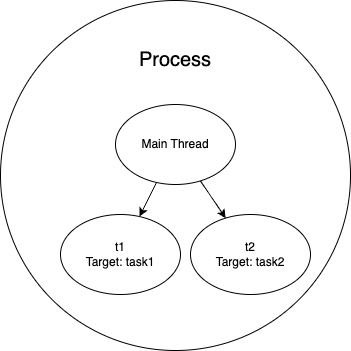
\includegraphics[width=0.5\textwidth]{b_class/asset/example.png}  % Sesuaikan nama file dan ukurannya
    \caption{Ini adalah gambar contoh dari multithreading.}
    \label{fig:contoh_gambar}
\end{figure}

Seperti yang terlihat pada Gambar \ref{fig:contoh_gambar}, inilah cara menambahkan gambar dengan keterangan.

\subsection{File Systems}
File systems provide a way for the operating system to store, retrieve, and manage data. This section explains:
\begin{itemize}
    \item File system structure
    \item File access methods
    \item Directory management
\end{itemize}

\subsection{Input and Output Management}
\subsubsection{Apa itu Manajemen I/O?}
Manajemen I/O merupakan entitas yang bertanggungjawab mengontrol perangkat eksternal dan untuk pertukaran data antar perangkat tersebut dengan memori dan CPU. Perangkat eksternal itu seperti keyboard, mouse dan lain sebagainya.
\subsubsection{Fungsi Utama Modul I/O}
Fungsi utama modul I/O dikategorikan menjadi 5(lima), yaitu:
\begin{itemize}
    \item Contol dan timing : Modul I/O berfungsi untuk mengatur aliran data antara sistem inti komputer (seperti CPU dan memori) dan perangkat eksternal. Fungsi ini membutuhkan control dan timing yang tepat, karena ada perbedaan kecepatan dan mekanisme antara CPU dan perangkat eksternal yang biasanya lebih lambat. Modul I/O harus memastikan bahwa data dikirim dan diterima sesuai dengan waktu yang tepat, tanpa menyebabkan konflik atau kerusakan data.
    \item Komunikasi CPU : Modul I/O harus mampu berkomunikasi baik dengan CPU maupun dengan perangkat eksternal. Komunikasi ini mencakup beberapa aspek:
    \begin{itemize}
    \item Command Decoding (Dekode Perintah): Modul I/O menerima perintah dari CPU, yang biasanya dikirim melalui sinyal pada bus kontrol. Contoh perintah untuk modul I/O pada disk adalah seperti READ SECTOR, WRITE SECTOR, SEEK nomor track, dan SCAN record ID. Beberapa perintah ini mungkin menyertakan parameter yang dikirim melalui bus data.
    \item Data: Data ditransfer antara CPU dan modul I/O melalui bus data. Ini adalah proses pertukaran data yang terjadi setelah perintah diterima dan diproses oleh modul I/O.
    \item Status Reporting (Laporan Status): Karena perangkat eksternal seringkali lebih lambat daripada CPU, modul I/O harus melaporkan statusnya kepada CPU, misalnya dengan sinyal status seperti BUSY (sibuk) atau READY (siap). Ini penting agar CPU tahu apakah modul I/O siap untuk melakukan operasi atau sedang sibuk dengan perintah lain.
    \item Address Recognition (Pengenalan Alamat): Sama seperti memori memiliki alamat unik, perangkat I/O juga memiliki alamat yang unik. Modul I/O harus mampu mengenali alamat unik dari perangkat-perangkat yang dikendalikannya untuk mengarahkan data ke perangkat yang benar.
    \end{itemize}
    \item Komunikasi Perangkat : Modul I/O juga harus bisa berkomunikasi langsung dengan perangkat eksternal. Komunikasi ini meliputi:
    \begin{itemize}
        \item Perintah (instruksi yang dikirim ke perangkat).
        \item Informasi Status (kondisi perangkat, seperti siap atau sibuk).
        \item Data (informasi yang ditransfer antara perangkat dan CPU).
    \end{itemize}
    \item Data Buffering : Modul I/O bertugas untuk menyiapkan data dari atau untuk perangkat eksternal melalui buffering (penyimpanan sementara data) sehingga data dapat diproses dengan lebih efisien, mengatasi perbedaan kecepatan antara CPU dan perangkat eksternal.
    \item Deteksi Error : Modul I/O juga bertanggung jawab untuk mendeteksi dan melaporkan kesalahan yang terjadi saat komunikasi dengan perangkat eksternal. Kesalahan ini bisa berupa masalah mekanis (seperti kertas yang menggulung pada printer) atau kesalahan elektris (seperti kesalahan bit saat mentransfer data). Modul I/O kemudian akan melaporkan kesalahan ini ke CPU agar dapat diatasi.
\end{itemize}
\subsubsection{Struktur Modul I/O}
\begin{figure}[h]
    \centering
    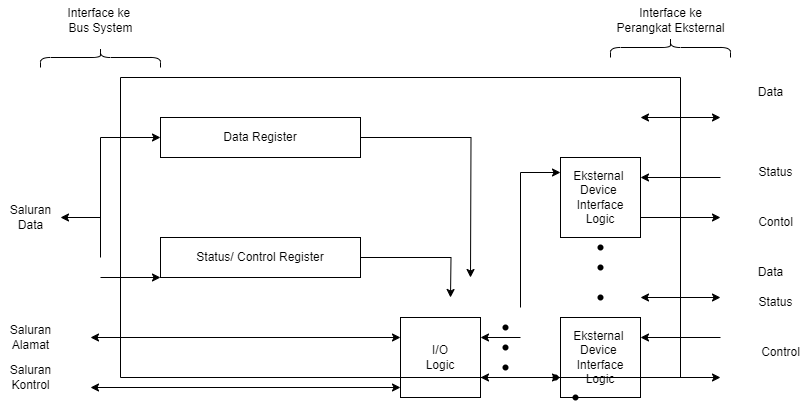
\includegraphics[width=0.80\linewidth]{b_class/asset/sisop.drawio.png}
    \caption{Struktur Modul I/O}
    \label{fig:enter-label}
\end{figure}
Penjelasan:
\begin{itemize}
    \item Data, alamat, dan kontrol dikirim dari sistem komputer (bus system) ke modul I/O.
    \item I/O Logic mengelola aliran data, kontrol, dan alamat yang masuk.
    \item Data Register menyimpan data sementara, dan Status/Control Register mengatur status dan kontrol perangkat.
    \item Eksternal Device Interface Logic menjembatani data, status, dan kontrol ke perangkat eksternal.
    \item Data, status, dan kontrol diolah dan dikirim ke perangkat eksternal, dan informasi status kembali ke sistem komputer.
\end{itemize}
\subsubsection{Control dan Timing}
\newline Control dan Timing berfungsi untuk mengatur agar kecepatan transfer, data yang berbeda-beda antar periferal dapat tersinkronisasi. Misalnya, kontrol pemindahan data dari sebuah perangkat eksternal ke CPU. Contoh kontrol pemindahan data dari sebuah perangkat eksternal ke CPU meliputi langkah-langkah berikut:
\begin{enumerate}
    \item CPU meminta modul I/O untuk memeriksa status perangkat yang terhubung.
    \item Modul I/O memberikan jawabannya tentang status perangkat.
    \item Bila perangkat sedang beroperasi dan berada dalam keadaan siap untuk mengirimkan, maka CPU meminta pemindahan data,dengan menggunakan perintah tertentu ke modul I/O..
    \item Modul I/O akan memperoleh unit data (misalnya, 8 atau 16 bit) dari perangkat eksternal.
    \item Data akan dipindahkan dari modul I/O ke CPU.
\end{enumerate}

\subsection{Deadlock Introduction and Prevention}
Explores the concept of deadlocks and methods for preventing them:
\begin{itemize}
    \item Deadlock conditions
    \item Deadlock prevention techniques
\end{itemize}

\subsection{User Interface Management}
This section discusses the role of the operating system in managing the user interface. Topics covered include:
\begin{itemize}
    \item Graphical User Interface (GUI)
    \item Command-Line Interface (CLI)
    \item Interaction between the user and the operating system
\end{itemize}

\subsection{Virtualization in Operating Systems}
Virtualization allows multiple operating systems to run concurrently on a single physical machine. This section explores:
\begin{itemize}
    \item Concept of virtualization
    \item Hypervisors and their types
    \item Benefits of virtualization in modern computing
\end{itemize}

\section{Assignments and Practical Work}
\subsection{Assignment 1: Process Scheduling}
Students were tasked with implementing various process scheduling algorithms (e.g., FCFS, SJN, and RR) and comparing their performance under different conditions.
\subsubsection{Group 1}
\begin{python}
    class Process:
    def __init__(self, pid, arrival_time, burst_time):
        self.pid = pid
        self.arrival_time = arrival_time
        self.burst_time = burst_time
        self.completion_time = 0
        self.turnaround_time = 0
        self.waiting_time = 0
\end{python}

\begin{table}[htbp] % Optional: For floating position
    \centering
    \begin{tabular}{|c|c|c|} % Defines number of columns and alignment (c = center, l = left, r = right). '|' creates vertical lines.
    \hline
    Header 1 & Header 2 & Header 3 \\ % Column headers
    \hline
    Row 1, Column 1 & Row 1, Column 2 & Row 1, Column 3 \\ % First row of data
    \hline
    Row 2, Column 1 & Row 2, Column 2 & Row 2, Column 3 \\ % Second row of data
    \hline
    \end{tabular}
    \caption{Your table caption} % Optional: For adding a caption
    \label{tab:your_label} % Optional: For cross-referencing the table
\end{table}

\subsection{Assignment 2: Deadlock Handling}
In this assignment, students were asked to simulate different deadlock scenarios and explore various prevention methods.

\subsection{Assignment 3: Multithreading and Amdahl's Law}
This assignment involved designing a multithreading scenario to solve a computationally intensive problem. Students then applied **Amdahl's Law** to calculate the theoretical speedup of the program as the number of threads increased.

\subsection{Assignment 4: Simple Command-Line Interface (CLI) for User Interface Management}
Students were tasked with creating a simple **CLI** for user interface management. The CLI should support basic commands such as file manipulation (creating, listing, and deleting files), process management, and system status reporting.

\subsection{Assignment 5: File System Access}
In this assignment, students implemented file system access routines, including:
\begin{itemize}
    \item File creation and deletion
    \item Reading from and writing to files
    \item Navigating directories and managing file permissions
\end{itemize}

\section{Conclusion}
The first half of the course introduced core operating system concepts, including process management, scheduling, multithreading, and file system access. These topics provided a foundation for more advanced topics to be covered in the second half of the course.

\end{document}